\chapter{Revisão Sistemática da Literatura em Transcodificação de Vídeo}
\label{cap:3}

O objetivo principal deste capítulo é apresentar ao leitor o estado da arte da literatura científica acerca de transcodificadores rápidos de vídeo. De forma a garantir uma maior acurácia da metodologia de pesquisa da literatura científica, utilizamos o processo de Metodologia Sistemática da Literatura (MSL) \cite{bib:msl}. Segundo essa metodologia, deve-se definir bem o escopo da busca pela literatura, a fim de possibilitar a replicação desse processo o mais fielmente possível, haja vista que é esperado que ocorra alguma mudança, pois a literatura é constantemente atualizada.

Assim sendo, nesta tese, utilizamos três ferramentas de busca como fonte dos artigos acadêmicos: a IEEE Xplore, a \textit{Association for Computing Machinery} (ACM) \textit{Library} e o \textit{Google Scholar}. Em cada uma delas, realizamos as mesmas buscas, procurando a presença das palavras ``\textit{transcoding}'' e ``\textit{transcoder}'', seja no título ou no \textit{abstract}. Selecionamos para estudo os primeiros 500 artigos que cada uma das ferramentas de busca considerou mais relevantes, totalizando 1500 artigos a serem revisados.

Após a obtenção dos artigos, aplicamos filtros para remover trabalhos com as características descritas abaixo: 

\begin{enumerate}[i.]
    \item Artigos duplicados;

    \item Artigos que focam na transcodificação de dados que não vídeo – por exemplo, transcodificação de áudio;

    \item Artigos que empregam o termo ``transcodificação'' como sinônimo para outra palavra, como ``codificação'';

    \item Artigos que apresentam a transcodificação sem foco em acelerar o processo, ou seja, não possuem redução do tempo (TS) ou qualquer forma de mensurar esse valor;

    \item Artigos que não apresentam a métrica BD-rate.
\end{enumerate}

Após os quatro primeiros filtros, dos 1500 artigos capturados sobraram 140; no entanto, somente 34 deles é que passaram pelo quinto filtro. Observe que o BD-rate começou a ser utilizado na literatura científica após o ano de 2010. Portanto, existe esse recorte dos trabalhos: consideramos apenas a última década (2011-2022) de artigos publicados com foco em acelerar a transcodificação de vídeo. Isso porque a ausência do BD-rate inviabiliza qualquer discussão comparativa entre os trabalhos. De cada um dos artigos selecionados, os seguintes dados foram capturados e armazenados em uma tabela:

\begin{enumerate}[1.]
    \item Título do artigo;
    
    \item Nome dos autores;
    
    \item Código do \textit{Digital Object Identifier} (DOI);
    
    \item Nome do formato utilizado na decodificação;
    
    \item Nome do formato utilizado na recodificação;
    
    \item Estágios envolvidos na transcodificação. Os possíveis estágios a serem selecionados neste campo são: ``predição intraquadro'', ``predição interquadros'', ``transformada'', ``quantização'', ``codificação de entropia'', ``filtros'', ``particionamento de blocos'' e ``outros'';
    
    \item Nome do algoritmo de aprendizado de máquina utilizado, quando existente;
    
    \item Breve descrição da proposta apresentada no trabalho.
\end{enumerate}

Com os artigos devidamente catalogados, torna-se possível apresentar o estado da arte da transcodificação de vídeo com foco na redução do custo computacional. Para facilitar essa apresentação, categorizamos os trabalhos em três tópicos: visão geral da transcodificação de vídeo (seção \ref{cap:3.1}); transcodificação assistida por aprendizado de máquina (seção \ref{cap:3.2}) e transcodificação acelerada por herança de particionamento de blocos (seção \ref{cap:3.3}).

Entre os trabalhos selecionados, é possível observar uma prevalência de soluções para transcodificação de ``origem'' ou para ``destino'' o formato H.265/HEVC. Aproximadamente 85\% de todos os trabalhos selecionados incluem soluções que visam adaptar vídeos codificados no padrão H.265/HEVC para tecnologias mais antigas (como H.264/AVC) ou para tecnologias mais recentes (como H.266/VVC). Tendo em vista que o escopo do estudo do estado da arte apresentado está entre os anos de 2011 e 2022, torna-se compreensível que o H.265/HEVC tenha sido o formato de vídeo mais estudado na literatura, pois o H.265/HEVC foi o padrão de codificação de vídeo estado-da-arte desde seu lançamento em 2013 até 2020, quando o H.266/VVC foi lançado. O segundo formato de vídeo que mais aparece na literatura selecionada é o H.264/AVC, com presença de 63\% entre todos os artigos, seguido pelo AV1 (15\%). Esses dois codificadores de vídeo são amplamente utilizados para fins comerciais hoje em dia, principalmente para transmissões de vídeos pela internet. Portanto, já esperávamos que tivessem destaque especial na literatura.

Considerando os tipos de transcodificações apresentados em \cite{bib:modosTranscodificacao} (vide Figura \ref{fig:4}), podemos encontrar, na literatura selecionada, dois tipos principais de trabalhos: transcodificações heterogêneas (78\%) e transcodificações homogêneas (22\%), sendo que esta última está subdividida em redução da taxa de bits (\textit{transrating}) e redução da resolução espacial (\textit{downscaling}). Dessa forma, essa diferença dos tipos de trabalho evidencia que a conversão entre formatos de vídeo é particularmente importante na literatura científica, assim como a adaptação da taxa de bits e o controle da resolução do vídeo, principalmente ao se considerar a relevância dos serviços de \textit{streaming} nos dias de hoje.

Dentre todos os formatos e padrões de codificação de vídeos apresentados na Figura \ref{fig:1}, encontram-se presentes na revisão sistemática da literatura apenas os formatos H.264/AVC, H.265/HEVC, H.266/VVC, VP9, AV1 e AVS, distribuídos conforme a Figura \ref{fig:10}. Em relação à transcodificação homogênea (Figura \ref{fig:10}(a)), encontramos apenas trabalhos que propõem soluções para os formatos H.264/AVC ou H.265/HEVC, sendo que este último representa 57,14\% dos casos. Para trabalhos de transcodificação de vídeos heterogêneos, H.264/AVC também é o principal formato de origem, com presença de 61,54\% (Figura \ref{fig:10}(b)), enquanto o formato H.265/HEVC é o principal formato de destino, com 65,38\% (Figura \ref{fig:10}(c)). Portanto, é possível notar que os formatos de codificação de vídeo desenvolvidos pelo ITU-VCEG têm sido o foco principal dos pesquisadores que trabalham com transcodificação de vídeo.

\begin{figure}
    \centering
    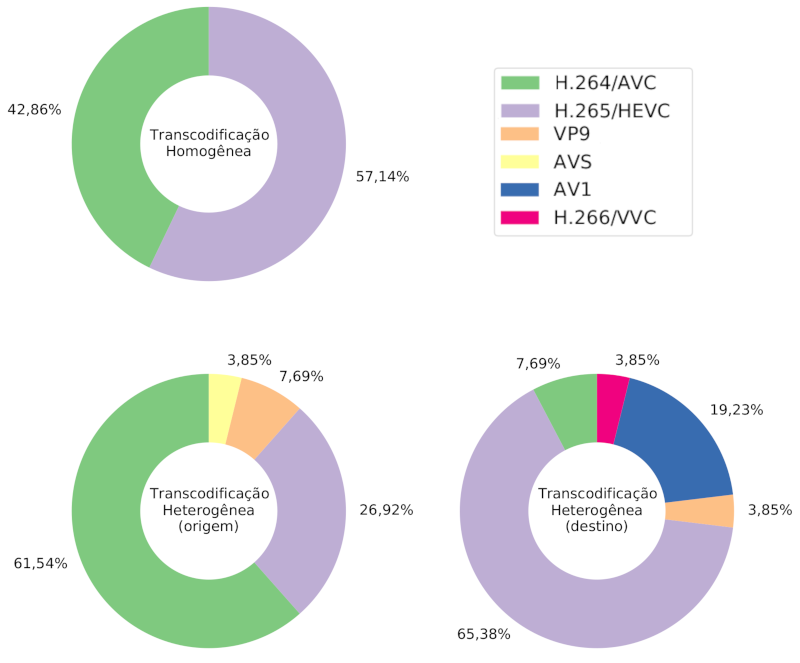
\includegraphics[width=\textwidth]{FIGURES/fig_10.png}
    \caption{Distribuição da presença dos formatos de codificação de vídeo observados na revisão sistemática da literatura, conforme o tipo de transcodificação. Fonte: Elaborada pelo autor.}
    \label{fig:10}
\end{figure}

Descrevemos os seis principais estágios de um codificador de vídeo híbrido no capítulo \ref{cap:2}, mas o particionamento de blocos também é um processo decisório importante durante a execução de um codificador. Portanto, precisa ser considerado quando se trata do estudo de complexidade daquele formato de codificação de vídeo. Ao observar a literatura selecionada, percebemos que a maioria das soluções concentram seus esforços em acelerar um transcodificador de vídeo através do processo de particionamento de blocos, como pode ser visto na Figura \ref{fig:11}. Nela, mostramos a distribuição do campo ``estágios envolvidos na transcodificação'', de acordo com os dados capturados durante a revisão da literatura. O círculo externo dessa figura representa todo o conjunto de 140 artigos revisados após os quatro primeiros processos de filtragem, ou seja, removidos os trabalhos duplicados e que não estão relacionados à transcodificação rápida de vídeo, enquanto o círculo interno representa o conjunto dos 34 artigos que, de fato, foram selecionados após o quinto processo de filtragem. Conforme mostrado no círculo interno, os estágios abordados no reaproveitamento de informações em soluções para transcodificação acelerada são: o particionamento de bloco (70,59\%), a predição interquadros (41,18\%) e a predição intraquadro (8,89\%). É notório nessa figura que os três principais tópicos de estudo são os mesmos nos dois círculos, mas com distribuições diferentes. Antes da aplicação dos dois últimos filtros, observamos outra ordem: predição interquadros (42,62\%), particionamento de blocos (18,58\%) e predição intraquadro (17,49\%).

\begin{figure}
    \centering
    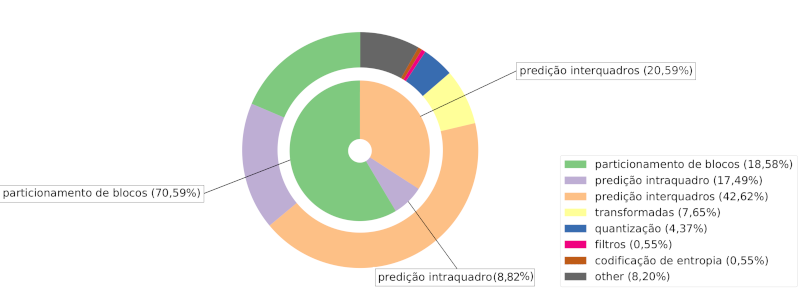
\includegraphics[width=\textwidth]{FIGURES/fig_11.png}
    \caption{Distribuição do campo ``estágios envolvidos na transcodificação'', observados durante a revisão sistemática da literatura. Fonte: Elaborada pelo autor.}
    \label{fig:11}
\end{figure}

Após essa visão geral dos trabalhos revisados, podemos apresentar, de forma mais especializada, cada um dos tópicos de interesse acerca do estado da arte em transcodificação rápida de vídeo.

\section{Visão Geral da Transcodificação Rápida de Vídeo}
\label{cap:3.1}

Os 34 artigos selecionados após as etapas de filtragem estão resumidos na Tabela \ref{tab:III}, apresentando os formatos de decodificação e de codificação utilizados, assim como as métricas BD-rate e TS para cada solução proposta. Todos eles fazem uso de heurísticas para acelerar o transcodificador, com base em análises estatísticas ou em aprendizado de máquina. Em média, os trabalhos de aceleração da transcodificação de vídeo publicados na última década são capazes de reduzir o tempo do processo de transcodificação à metade (TS médio igual à 50,74\%) em comparação com o transcodificador original correspondente. Observando o desvio padrão da redução do tempo, é seguro afirmar que existe uma grande probabilidade de que soluções de transcodificação rápida ofereçam uma redução de tempo entre 31,51\% e 69,97\%. Já o impacto médio na eficiência de codificação (em termos de BD-rate) é de 4,11\%, e não superior a 6,57\% em média (considerando desvio padrão mais a média), indicando que é esperada alguma perda na eficiência de codificação, desde pequenos a médios valores de BD-rate, ao se executar a transcodificação na metade do tempo de um transcodificador original.

\afterpage{
\clearpage

\begin{landscape}
{\footnotesize
\begin{longtblr}[
    caption = {Resumo dos artigos presentes na revisão sistemática da literatura sobre transcodificação rápida de vídeo, publicados entre os anos de 2011 e 2022.},
    label = {tab:III},
    note{1} = {Valor adaptado da métrica ``número de vezes mais rápido que'' (do inglês, \textit{speed-up}) para percentual TS.}
]{
    colspec = {p{5cm}|p{2.2cm}|p{2.2cm}|p{4cm}|c|c|c},
    rowhead = 1,
    hlines,
    row{even} = {gray9}
}
\hline
\textbf{Autor} & \textbf{Formato de Origem} & \textbf{Formato de Destino} & \textbf{Estágios Envolvidos} & \textbf{BD-rate (\%)} & \textbf{TS (\%)} & \textbf{Razão ($\frac{BD-rate}{TS}$)} \\
\citet{bib:leuven_2011} & H.264/AVC & H.264/AVC & particionamento de blocos, predição intraquadro & 7,33 & 95,73 & 0,077 \\
\citet{bib:wang_2012} & H.264/AVC & H.264/AVC & predição interquadros & 3,53 & 90,62 & 0,039 \\
\citet{bib:aminlou_2016} & H.264/AVC & H.264/AVC & predição interquadros & 6,60 & 6,80 & 0,971 \\
\SetCell[c=4]{r}\textit{Média de H.264/AVC-to-H.264/AVC} &&&& \textit{5.82} & \textit{64.38} & \\
\SetCell[c=4]{r}\textit{Desvio Padrão de H.264/AVC-to-H.264/AVC} &&&& \textit{2,02} & \textit{49,93} & \\

\citet{bib:zhang_2012} & H.264/AVC & H.265/HEVC & particionamento de blocos, predição intraquadro e predição interquadros & 30,00 & 80,00 & 0,375 \\
\citet{bib:peixoto_2012} & H.264/AVC & H.265/HEVC & predição interquadros & 5,49 & 52,74 & 0,104 \\
\citet{bib:jiang_2013} & H.264/AVC & H.265/HEVC & predição interquadros & 1,45 & 30,50 & 0,048 \\
\citet{bib:peixoto_2014} & H.264/AVC & H.265/HEVC & predição interquadros & 3,87 & 63,06 & 0,061 \\
\citet{bib:peixoto2_2014} & H.264/AVC & H.265/HEVC & particionamento de blocos & 8,41 & 70,54 & 0,119 \\
\citet{bib:honrubia_2014} & H.264/AVC & H.265/HEVC & particionamento de blocos & 4,80 & 64,29 & 0,075 \\
\citet{bib:peixoto3_2014} & H.264/AVC & H.265/HEVC & particionamento de blocos, predição intraquadro e predição interquadros & 3,32 & 49,75\TblrNote{1} & 0,067 \\
\citet{bib:nagaraghatta_2015} & H.264/AVC & H.265/HEVC & predição interquadros & 4,20 & 50,33 & 0,083 \\
\citet{bib:franche_2015} & H.264/AVC & H.265/HEVC & BP. predição interquadros & 3,28 & 87,32 & 0,038 \\
\citet{bib:honrubia_2015} & H.264/AVC & H.265/HEVC & particionamento de blocos & 5,20 & 60,00\TblrNote{1} & 0,087 \\
\citet{bib:honrubia_2016} & H.264/AVC & H.265/HEVC & particionamento de blocos & 2,20 & 57,37 & 0,038 \\
\citet{bib:correa_2016} & H.264/AVC & H.265/HEVC & particionamento de blocos & 1,67 & 44,10 & 0,038 \\
\citet{bib:franche_2017} & H.264/AVC & H.265/HEVC & predição interquadros & 10,13 & 67,90 & 0,149 \\
\citet{bib:liu_2018} & H.264/AVC & H.265/HEVC & particionamento de blocos & 1,83 & 53,71 & 0,034 \\
\citet{bib:xu_2019} & H.264/AVC & H.265/HEVC & particionamento de blocos & 1,16 & 59,60 & 0,019 \\
\citet{bib:soares_2019} & H.264/AVC & H.265/HEVC & particionamento de blocos & 0,75 & 24,28 & 0,031 \\
\citet{bib:xin_2022} & H.264/AVC & H.265/HEVC & particionamento de blocos & 0,60 & 38,40 & 0,015 \\
\SetCell[c=4]{r}\textit{Média de H.264/AVC-to-H.265/HEVC} &&&& \textit{5,20} & \textit{56,11} \\
\SetCell[c=4]{r}\textit{Desvio Padrão de H.264/AVC-to-H.265/HEVC} &&&& \textit{2,71} & \textit{15,59} \\

\citet{bib:sung_2014} & H.265/HEVC & H.265/HEVC & particionamento de blocos & 1,46 & 51,02 & 0,029 \\
\citet{bib:nguyen_2015} & H.265/HEVC & H.265/HEVC & particionamento de blocos & 0,88 & 40,50 & 0,022 \\
\citet{bib:grellert_2018} & H.265/HEVC & H.265/HEVC & particionamento de blocos & 0,29 & 41,81 & 0,007 \\
\citet{bib:lindino_2021} & H.265/HEVC & H.265/HEVC & particionamento de blocos & 0,54 & 42,00 & 0,013 \\
\citet{bib:xin_2022} & H.265/HEVC & H.265/HEVC & particionamento de blocos & 0,60 & 38,40 & 0,015 \\
\SetCell[c=4]{r}\textit{Média de H.265/HEVC-to-H.265/HEVC} &&&& \textit{5.20} & \textit{56,11} \\
\SetCell[c=4]{r}\textit{Desvio Padrão de H.265/HEVC-to-H.265/HEVC} &&&& \textit{2,71} & \textit{15,59} \\

\citet{bib:borges_2019} & H.265/HEVC & AV1 & particionamento de blocos & 4,55 & 35,41 & 0,128 \\
\citet{bib:borges2_2019} & H.265/HEVC & AV1 & particionamento de blocos & 4,94 & 35,43 & 0,139 \\
\citet{bib:chen_2019} & H.265/HEVC & AV1 & particionamento de blocos & 0,79 & 37,80 & 0,021 \\
\citet{bib:borges2_2021} & H.265/HEVC & AV1 & particionamento de blocos & 5,38 & 34,06 & 0,158 \\
\SetCell[c=4]{r}\textit{Média de H.265/HEVC-to-AV1} &&&& \textit{3,91} & \textit{35,68} \\
\SetCell[c=4]{r}\textit{Desvio Padrão de H.265/HEVC-to-AV1} &&&& \textit{2,11} & \textit{1,56} \\

\citet{bib:jin_2011} & AVS & H.264/AVC & predição intraquadro e predição interquadros & 0,58 & 78,15 & 0,007 \\
\citet{bib:tang_2015} & H.265/HEVC & H.264/AVC & particionamento de blocos, predição intraquadro e predição interquadros & 2,68 & 60,62 & 0,044 \\
\citet{bib:torre_2015} & H.265/HEVC & VP9 & predição interquadros & 3,51 & 36,24 & 0,097 \\
\citet{bib:li_2017} & VP9 & H.265/HEVC & particionamento de blocos & 3,70 & 43,50 & 0,085 \\
\citet{bib:lucas_2020} & H.265/HEVC & H.266/VVC & particionamento de blocos & 0,32 & 13,38 & 0,024 \\
\citet{bib:borges_2021} & VP9 & AV1 & particionamento de blocos & 4,34 & 28,16 & 0,154 \\
\SetCell[c=4]{r}\textbf{Média Geral} &&&& \textbf{4,11} & \textbf{50,74} \\
\SetCell[c=4]{r}\textbf{Desvio Padrão Geral} &&&& \textbf{2,46} & \textbf{19,23} \\
\hline
\end{longtblr}
}
\end{landscape}
}


Há propostas de transcodificação rápida que não estão dentro da faixa média $\pm$ desvio padrão, podendo apresentar resultados tanto positivos como negativos em relação à média. Todavia, sem haver uma análise crítica em relação aos parâmetros de configurações utilizadas por essas propostas, assim como os contextos de aplicação de cada uma das técnicas utilizadas nestas propostas, qualquer valor observado de BD-rate e TS não pode ser comparado com essa média da literatura sem ocasionar em injustiças. Dessa forma, a média observada na literatura serve apenas como uma referência probabilistica. Por exemplo, \citet{bib:jin_2011} apresenta um valor significativamente positivo ao transcodificar de AVS-para-H.264/AVC, pois sua proposta atinge uma redução de tempo de 78,15\% com uma mínima perda de eficiência de compressão (0,58\% de BD-rate). Em \citet{bib:jin_2011}, os autores propõem um \textit{downscaling} de resolução de vídeo codificado originalmente em AVS para o padrão H.264/AVC ao mapear a predição intraquadro, ou seja, propõem aplicar uma transcodificação homogênea e heterogênea ao mesmo tempo. Por outro lado, um resultado considerado negativo pode ser observado em \citet{bib:leuven_2011}, que limita a predição intraquadro e o particionamento de blocos sob certas condições. Nesse trabalho, há uma equivalência percentual entre os valores de redução de tempo e de impacto na eficiência de codificação (TS=6,8\% e BD-rate=6,6\%), o que indica uma baixa relação entre eficiência de codificação e aceleração. Isso pode ser observado na coluna Razão, na qual valores próximos de zero são ideais, pois indicam um leve aumento na taxa de BD-rate para cada ponto percentual de aceleração obtido. Além disso, essa coluna permite equacionar diferentes soluções de forma mais direta, tornando possível compará-las. Por exemplo, as soluções propostas por \citet{bib:franche_2015}, \citet{bib:honrubia_2016} e \citet{bib:correa_2016}, todas com foco na transcodificação de H.264/AVC para H.265/HEVC, apresentam resultados diferentes de BD-rate (3,28\%, 2,20\% e 1,70\%, respectivamente) e de TS (87,32\%, 57,37\% e 44,10\%, respectivamente), no entanto, são similares, já que possuem a mesma razão de 0,038.

A Figura \ref{fig:12} apresenta os trabalhos da Tabela \ref{tab:III} espalhados visualmente, onde cada ponto indica um trabalho indicado pela primeira letra do sobrenome do autor seguido do ano de publicação do trabalho; nela, o eixo horizontal representa a perda de eficiência de codificação (BD-rate) e o eixo vertical, a aceleração de transcodificação (TS). O gráfico permite visualizar os dados da Tabela \ref{tab:III}. No entanto, é de suma importância enfatizar que qualquer comparação direta entre os trabalhos não é possível, ou mesmo justa, apenas avaliando os seus resultados de BD-rate e TS, sem que se faça uma distinção entre contextos e aplicabilidades. Avaliando-se a Figura \ref{fig:12}, poderia-se supor que os pontos mais próximos da região superior esquerda forneçam as melhores relações entre redução de complexidade e eficiência de codificação, ou seja, são propostas que apresentam baixa Razão, que vai aumentando conforme os resultados se afastam dessa região. Nesta visão mais ampla, os resultados que apresentam as melhores relações de Razão foram obtidos por \citet{bib:jin_2011} e \citet{bib:grellert_2018}, todos eles com uma Razão de 0,007. Por outro lado, as duas propostas com maior Razão são \citet{bib:aminlou_2016} (Razão de 0,971) e \citet{bib:zhang_2012} (Razão de 0,375). Para melhor visualização, o trabalho de \citet{bib:zhang_2012} não foi incluído na Figura \ref{fig:12} devido ao alto valor de BD-rate (30\%).

\afterpage{
\clearpage
\begin{landscape}
\begin{figure}
    \centering
    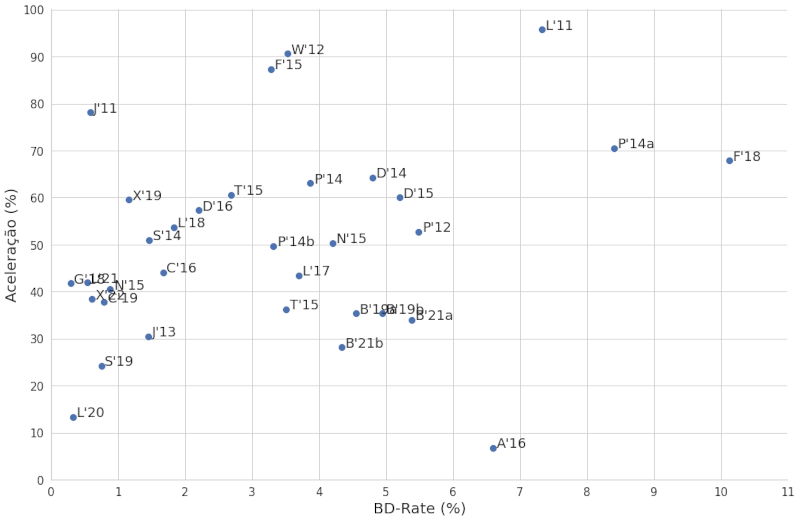
\includegraphics[width=0.8\linewidth]{FIGURES/fig_12.png}
    \caption{Valores de redução do tempo e do impacto na eficiência de codificação dos trabalhos selecionados pela revisão sistemática da literatura. Fonte: Elaborada pelo autor.}
    \label{fig:12}
\end{figure}
\end{landscape}
}


Uma análise mais aprofundada dos artigos apresentados na Tabela \ref{tab:III} permite observar que a reutilização do particionamento de blocos é a estratégia preferida para acelerar o processo de transcodificação, principalmente após o ano de 2015. Isso pode ser explicado porque o particionamento de blocos é uma tarefa essencial na codificação de vídeo, representando o principal laço de repetição do complexo processo de Otimização Taxa-Distorção (do inglês, \textit{Rate-Distortion Optimization}, RDO) \cite{bib:rdo_sullivan}, com decisões que afetam todos os estágios de codificação, direta ou indiretamente. A seção \ref{cap:3.3} cobre com mais detalhes essa categoria de soluções.

Por fim, é perceptível que a perda de eficiência de compressão diminuiu significativamente nos trabalhos publicados nos últimos anos. De fato, 70\% dos artigos da Tabela \ref{tab:III} que atingem um BD-rate inferior a 3\% empregam soluções baseadas em aprendizado de máquina para acelerar as decisões de transcodificação. Por essa razão, discutimos essa categoria de forma mais minuciosa na seção \ref{cap:3.2}.

\section{Transcodificação Assistida por Aprendizado de Máquina}
\label{cap:3.2}

O aprendizado de máquina (do inglês, \textit{Machine Learning}, ML) é um campo de pesquisa que cresceu significativamente nos últimos anos e hoje é aplicado em diversas áreas para resolver diferentes tipos de problema. Na área de codificação de vídeo, isso não é diferente, com contribuições que vão desde o desenvolvimento de novas ferramentas baseadas em aprendizado para codecs híbridos até autoencoders \cite{bib:autoencoder}, codificadores de vídeo totalmente baseados em redes neurais profundas. Quanto às soluções de transcodificação rápida, as propostas são tipicamente focadas em auxiliar as tomadas de decisão, baseando-se em dados extraídos do \textit{bitstream} decodificado e evitando, assim, o teste exaustivo do RDO para várias possibilidades de codificação. Nessas propostas, incluem-se decisões sobre: os modos de predição, a geração de vetores de movimento e a pré-definição de particionamento de blocos. Essa simplificação do processo RDO pode ser tratada como um problema de classificação, pois o modelo treinado poderá detectar: 

\begin{enumerate}[i.]
    \item um modo único a ser testado, descartando todos os restantes;
    
    \item um modo único a ser descartado, testando os demais;
    
    \item um subconjunto de modos a serem testados, descartando os demais.
\end{enumerate}

Algumas soluções de transcodificação assistida por aprendizado de máquina também são baseadas em acelerações locais no lado do codificador, usando modelos treinados com informações obtidas tanto do decodificador (formato de origem) quanto do codificador (formato de destino). Por exemplo, além dos atributos reunidos durante a decodificação, \citet{bib:lucas_2020} também usa a média e a variância dos blocos residuais obtidos durante o processo de codificação do H.266/VVC para prever o particionamento do bloco a ser utilizado. O uso de reaproveitamento de dados de origem tanto do decodificador como do codificador também pode ser observado nos trabalhos de \citet{bib:nguyen_2015}, \citet{bib:franche_2015} e \citet{bib:franche_2017}, apesar de eles não utilizarem soluções baseadas em aprendizado de máquina. Em relação ao conjunto de atributos para serem processados pelo modelo de ML, podem ser diferentes ou idênticos, mesmo para prever decisões distintas. Por exemplo, \citet{bib:peixoto_2014} e \citet{bib:li_2017} usam o mesmo conjunto de recursos em seus trabalhos. Todavia, \citeauthor{bib:peixoto_2014} os usa para prever vetores de movimento a serem utilizados no H.264/AVC, enquanto \citeauthor{bib:li_2017} utiliza esses atributos para prever o particionamento de blocos na codificação H.265/HEVC.

As soluções apresentadas nesses artigos são baseadas em diversos métodos e algoritmos de aprendizado de máquina atualmente disponíveis. As contribuições desses trabalhos na transcodificação de vídeo estão resumidas na Figura \ref{fig:13}, categorizadas de acordo com o algoritmo empregado. No círculo externo da Figura \ref{fig:13}, está a distribuição das categorias de aprendizado de máquina, enquanto, no círculo interno, está a distribuição dos algoritmos utilizados. As soluções observadas na revisão sistemática da literatura se enquadram em três categorias principais de aprendizado de máquina supervisionado \cite{bib:livroKubat}: classificação linear, árvores de decisão e aprendizado profundo, como já foi apresentado na subseção \ref{cap:2.3}.

\begin{figure}
    \centering
    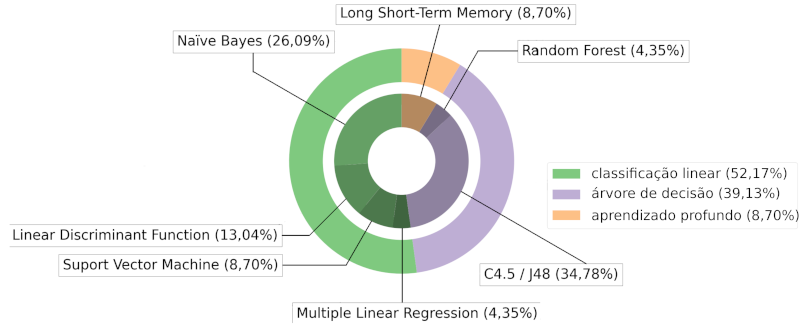
\includegraphics[width=\textwidth]{FIGURES/fig_13.png}
    \caption{Distribuição de algoritmos de aprendizado de máquina nos artigos revisados sobre aceleração de transcodificação de vídeo. Fonte: Elaborada pelo autor.}
    \label{fig:13}
\end{figure}

É possível observar, na Figura \ref{fig:13}, que o algoritmo C4.5/J48, dentro da categoria de árvores de decisão, é o mais empregado nas soluções encontradas na literatura. Por exemplo, \citet{bib:correa_2016} propõe o uso de árvores de decisão treinadas em C4.5 para prever o melhor particionamento de blocos para \textit{Coding Units} (CUs) do H.265/HEVC com base em dados coletados da decodificação do H.264/AVC. Da mesma forma, \citet{bib:escribano3_2008} emprega o mesmo algoritmo de ML para prever vetores de movimento na transcodificação de H.263 para VP6. Já \citet{bib:grellert_2018} usa modelos de \textit{Random Forest} para prever as profundidades máxima e mínima da estrutura de particionamento do H.265/HEVC para acelerar a codificação para aplicativos em tempo real.

Apesar de a categoria de árvores de decisão representar 39,13\% dos trabalhos, não é a mais comum observada na literatura. Conforme a Figura \ref{fig:13}, a categoria de classificadores lineares é a que apresenta maiores contribuições à literatura, totalizando 52,17\% dos trabalhos com uso de aprendizado de máquina. Dentro dessa categoria, \textit{Naïve-Bayes} é o algoritmo mais empregado, seguido por \textit{Linear Discriminant Functions} (LDF), \textit{Support Vector Machine} (SVM) e \textit{Multiple Linear Regression} (MLR). Como já foi dito, esses algoritmos geram modelos classificadores probabilísticos simples e eficientes \cite{bib:naivebayesref} e são amplamente utilizados porque demonstram precisão relevante mesmo para um pequeno conjunto de dados de treinamento. Dentre os trabalhos que fazem uso de \textit{Naïve-Bayes}, temos o de \citet{bib:honrubia_2016}, que propõe um transcodificador H.264/AVC-to-H.265/HEVC que faz uso do modelo para decidir sobre a predição intraquadro e o particionamento de bloco. Estratégia similar é encontrada no trabalho de \citet{bib:li_2017}, ao transcodificar vídeos de VP9 para o padrão H.265/HEVC.

Os últimos algoritmos de aprendizado de máquina que encontramos na literatura revisada se enquadram na categoria de aprendizado profundo. Há poucos trabalhos que implementam soluções a partir deste tipo de algoritmo de aprendizado de máquina, e isso era, de alguma forma, esperado, pois as soluções de aprendizado profundo geralmente exigem recursos computacionais expressivos tanto para o treinamento quanto para sua execução, o que tende a ser contraditório numa proposta de aceleração do transcodificador. Mesmo assim, a abordagem baseada no algoritmo \textit{Long Short-Term Memory} (LSTM) \cite{bib:graves_2012} foi proposta por \citet{bib:xu_2019} para acelerar a transcodificação H.264/AVC-para-H.265/HEVC, levando em consideração vários quadros decodificados do H.264/AVC para predizer sobre o particionamento de blocos do H.265/HEVC e obtendo uma aceleração de 59,6\% no tempo de transcodificação.

Ao utilizar algoritmos de aprendizado de máquina, para realizar a aceleração da transcodificação ou não, é imperativo escolher atributos que representem as informações de modo a auxiliar o modelo a retornar a melhor resposta. Como já vimos nesta seção, os mesmos atributos podem ser utilizados para diferentes fins, e não há consenso sobre quantos ou quais atributos devem ser usados para possibilitar um bom treinamento de modelo. Contudo, de forma genérica, a coleta de um maior número possível de atributos pode ser interessante, cabendo ao algoritmo de aprendizado de máquina decidir quais deles deverão ser levados em consideração durante a previsão. Ao mesmo tempo, é importante ressaltar que o aumento significativo de atributos torna mais complexo o processo de treinamento dos modelos. Ainda assim, considerando todos os artigos revisados que usam estratégias baseadas em aprendizado de máquina, encontramos trabalhos que utilizam menos de uma dezena de atributos e outros que utilizam mais de uma centena.

Para facilitar esse tipo de comparação, apresentamos a Tabela \ref{tab:IV}, que resume a literatura científica que faz uso de modelos de aprendizado de máquina. A Tabela \ref{tab:IV} apresenta ainda o algoritmo de ML utilizado em cada um dos trabalhos destacados na tabela, o estágio da codificação em que foi realizado o reaproveitamento de informação e uma breve descrição dos atributos selecionados. Note que os primeiros nove trabalhos apresentados na Tabela \ref{tab:IV} não fazem parte dos artigos selecionados na revisão sistemática da literatura, pois não apresentam resultados de BD-rate. Todavia, achamos pertinente apresentá-los nesta seção, a fim de possibilitar melhor compreensão do uso de algoritmos de ML em trabalhos de transcodificação de vídeo.

\afterpage{
\clearpage

\begin{landscape}
{\footnotesize
\begin{longtblr}[
    caption = {Resumo das abordagens baseadas em aprendizado de máquina encontradas na literatura para aceleração de transcodificadores de vídeo.},
    label = {tab:IV},
    note{1} = {Este artigo não apresenta resultados de BD-rate.},
    note{2} = {\citet{bib:huangyuan_2015} apresenta resultados de BD-PSNR ao invés de BD-rate.}
]{
    colspec = {p{2.8cm}|p{2cm}|p{3.3cm}|p{1.5cm}|p{13.4cm}},
    rowhead = 1,
    hlines,
    row{even} = {gray9}
}
 \hline
 \textbf{Autor} & \textbf{Algoritmo de ML} & \textbf{Estágios Envolvidos} & \textbf{Número de Atributos} & \textbf{Descrição dos Atributos Utilizados}\\
 
 %2006
 \citet{bib:fernandez2_2006}\TblrNote{1} & J48 & predição interquadros & 292 & Média ($\mu$) e variância ($\sigma^2$) dos blocos residuais de tamanho 4$\times$4; modo de predição no macrobloco (MB); modo de predição interquadros; modo do \textit{Coded Block Pattern} (CBP) do H.262/MPEG-2; modo equivalente ao CBP do H.264/AVC; MB residual quando o vetor de movimentos (VM) do H.262/MPEG-2 é considerado. \\
 
 %2007
 \citet{bib:wang2_2007}\TblrNote{1} & MLR & predição interquadros & 42 & vetores de movimento\\
 
 %2008
 \citet{bib:escribano3_2008}\TblrNote{1} & C4.5 & predição interquadros & 34 & $\mu$ e $\sigma^2$ do bloco residual de tamanho 4$\times$4; VM; modo de predição no MB; CBP. \\
 
 %2008
 \citet{bib:escribano3_2008}\TblrNote{1} & C4.5 & predição interquadros & 12 & $\mu$ e $\sigma^2$ do bloco residual de tamanho 8$\times$8 e 16$\times$16; CBP; erro absoluto quando VM=(0,0). \\
 
 %2008
 \citet{bib:escribano_2008}\TblrNote{1} & C4.5 & predição interquadros & 34 & $\mu$ e $\sigma^2$ do bloco residual de tamanho 4$\times$4; VM; modo de predição no MB; CBP. \\
 
 %2008
 \citet{bib:escribano2_2008}\TblrNote{1} & J48 & predição interquadros & 34 & $\mu$ e $\sigma^2$ do bloco residual de tamanho 4$\times$4; VM; modo de predição no MB; CBP. \\
 
 %2009
 \citet{bib:holder_2009}\TblrNote{1} & J48 & predição interquadros & 291 & $\mu$ e $\sigma^2$ do bloco residual de tamanho 4$\times$4; $\mu$ do bloco residual de tamanho 16$\times$16; CBP; coeficientes da transformada. \\
 
  %2015
 \citet{bib:huangyuan_2015}\TblrNote{2} & SVM & particionamento de blocos & 8 & soma e a $\sigma^2$ dos blocos residuais de tamanho 64$\times$64 e 32$\times$32; soma do bloco residual de tamanho 16$\times$16; modo de predição do MB; tipo de estrutura de particionamento; parâmetro de quantização. \\
 
 %2017
 \citet{bib:wei_2017}\TblrNote{1} & LSTM & particionamento de blocos & 3 & \textit{bitrate}, bloco residual; particionamento do MB. \\
 
 %2014
 \citet{bib:peixoto_2014} & LDF & predição interquadros & 15 & $\sigma^2$ da fase do VM; número de coeficientes da transformada; energia dos coeficientes da transformada; para cada tamanho de CU, sinais de uso do: modo SPLIT, modo SKIP da predição interquadros e do modo 2N$\times$2N da PU. \\
 
 %2014
 \citet{bib:peixoto2_2014} & LDF & particionamento de blocos & 10 & $\sigma^2$ da distância dos VM; $\sigma^2$ da fase do VM; número de coeficientes da transformada; distribuição dos modos de predição do H.264/AVC. \\
 
 %2014
 \citet{bib:honrubia_2014} & NB & particionamento de blocos & 25 & soma, $\mu$ e $\sigma^2$ dos elementos do VM; $\mu$ e $\sigma^2$ da CTU residual; $\mu$ e $\sigma^2$ da CU residual; soma horizontal e vertical dos filtros de Sobel; resolução do vídeo; nível de quantização; \textit{bitrate} da CTU; de cada quadro do vídeo, número de: modos de predição intraquadro, modos SKIP da predição interquadros, predições interquadros no bloco de tamanho 16$\times$16, predições interquadros no bloco de tamanho diferente de 16$\times$16, número de coeficientes da transformada diferente de zero de cada CTU. \\
 
 %2014
 \citet{bib:peixoto3_2014} & LDF & particionamento de blocos & 10 & $\sigma^2$ da distância e das fases do VM; número de coeficientes da transformada; distribuição dos modos de predição do H.264/AVC. \\
 
 %2015
 \citet{bib:honrubia_2015} & NB & particionamento de blocos & 27 & soma, $\mu$ e $\sigma^2$ dos elementos do VM; $\mu$ e $\sigma^2$ da CTU e da CU residual; soma horizontal e vertical dos filtros de Sobel; resolução do vídeo; nível de quantização; \textit{bitrate} da CTU; Lagrangiana do modo SKIP da predição interquadros e dos modos 2N$\times$2N da PU; de cada quadro do vídeo, número de: modos de predição intraquadro, modos SKIP da predição interquadros, predições interquadros no bloco de tamanho 16$\times$16, predições interquadros no bloco de tamanho diferente de 16$\times$16, número de coeficientes da transformada diferente de zero de cada CTU. \\
 
 %2016
 \citet{bib:honrubia_2016} & NB & particionamento de blocos predição intraquadro & 21 & $\mu$ e $\sigma^2$ of residual MB; $\mu$ e $\sigma^2$ of residual CU; number of intra predicted blocks with: horizontal, vertical, diagonal, DC e Planar modes; sum of intra predicted samples within a MB; number of non-zero transform coefficients; video resolution; QP; bitrate; sum of horizontal Sobel Filter; sum of vertical Sobel Filter. \\
 
 %2016
 \citet{bib:correa_2016} & C4.5 & particionamento de blocos & 33 & soma e $\mu$ dos blocos preditos; soma, $\mu$ e número de coeficientes da transformada; sinal de uso do modo SKIP da predição interquadros para os blocos 64$\times$64, 32$\times$32 e 16$\times$16; modo de predição intraquadro para os blocos 64$\times$64, 32$\times$32 e 16$\times$16; modo de predição no MB; CBP dos blocos de crominância. \\
 
 %2017
 \citet{bib:li_2017} & NB & particionamento de blocos & 74 & soma, $\mu$ e $\sigma^2$ dos elementos do VM; custo da taxa-distorção dos modos 2N$\times$2N da PU e dos modos SKIP da predição interquadros; número de blocos dentro de cada superbloco; mapa de profundidade da estrutura de particionamento. \\
 
  %2018
 \citet{bib:liu_2018} & SVM & particionamento de blocos & 3 & $\mu$ do \textit{bitrate}; $\mu$ absoluta dos blocos residuais; número de blocos dentro de cada CTU. \\
 
  %2018
 \citet{bib:grellert_2018} & RF & particionamento de blocos & 19 & modo de predição; modo da PU; profundidade da CU; coeficientes da transformada antes e depois da quantização; soma dos pixeis preditos; magnitude do VM. \\
 
 %2019
 \citet{bib:xu_2019} & LSTM & particionamento de blocos & 12 & VM; bloco residual; particionamento da MB; \textit{bitrate}. \\

 %2019
 \citet{bib:soares_2019} & J48 & particionamento de blocos & 13 & soma e $\mu$ dos coeficientes da transformada; soma e $\mu$ das amostras preditas nos blocos; tipo e posição do MB; CBP das camadas de crominância; sinal de uso do modo SKIP da predição interquadros; sinal de uso de algum modo de predição intraquadro; modo de predição intraquadro usado no bloco de tamanho 16$\times$16. \\
 
  %2019
 \citet{bib:chen_2019} & NB & particionamento de blocos & 3 & profundidade da CU; número de blocos em cada nível de profundidade em cada quadro; número de blocos em cada quadro. \\
 
 %2020
 \citet{bib:lucas_2020} & NB & particionamento de blocos & 16 & $\mu$ e $\sigma^2$ dos coeficientes assimétricos de Fisher e dos coeficientes de Kurtosis nos blocos residuais e reconstruídos para os blocos de tamanho 128$\times$128; $\mu$ das $\sigma^2$ e $\sigma^2$ das $\sigma^2$ dos blocos residuais e reconstruídos para os blocos de tamanho 64$\times$64; número de resíduos iguais a zero dentro do bloco de tamanho 128$\times$128; informação espacial dos blocos residuais de tamanho 128$\times$128; $\mu$ do desvio absoluto entre o bloco residual e o bloco reconstruído; \textit{bitrate}; produto da resolução do vídeo; função lambda entre o nível de quantização utilizado e o valor do grupo de quadros (\textit{group of pictures}, GoP).\\
 \hline
\end{longtblr}
}
\end{landscape}
}


A Tabela \ref{tab:IV} mostra que os artigos revisados empregam diversas informações como atributos. Por exemplo, a média ($\mu$) e a variância ($\sigma^2$) do bloco residual são frequentemente usadas como atributos, como visto em \citet{bib:fernandez2_2006}, \citet{bib:holder_2009}, \citet{bib:huangyuan_2015}, e \citet{bib:honrubia_2015}. Além disso, é possível encontrar atributos baseados em algum tipo de informação oriundo do vetor de movimento (do inglês, \textit{motion vector}, VM), como o VM de blocos 4$\times$4 (em \citet{bib:escribano3_2008}) e a variância das distâncias de VM (em \citet{bib:peixoto2_2014}, \citet{bib:honrubia_2014} e \citet{bib:li_2017}). O modo de predição intraquadro (em \citet{bib:honrubia_2016} e \citet{bib:soares_2019}), os parâmetros de predição interquadros (em \citet{bib:correa_2016}, \citet{bib:honrubia_2015}) e estruturas de particionamento de blocos (em \citet{bib:grellert_2018} e \citet{bib:xu_2019}) também são atributos frequentemente considerados para treinar modelos de aprendizado de máquina. Além disso, diversas métricas estatísticas como média e desvio padrão de diferentes características são amplamente empregadas, pois permitem representar tendências gerais no conjunto de dados disponíveis.

Ao analisarmos cuidadosamente os estágios envolvidos no processo de reaproveitamento presente na Tabela \ref{tab:IV}, percebemos que as estruturas de particionamento são as principais informações reaproveitadas nos trabalhos presentes na revisão sistemática da literatura. Sejam informações como tamanhos de blocos, orientações dos blocos ou árvores de particionamento, esses dados são atributos comumente utilizados em trabalhos de aprendizado de máquina (junto com informações oriundas de vetor de movimento). Por isso, a seção \ref{cap:3.3} detalha, particularmente, os artigos que se encontram nessa subcategoria.

\section{Transcodificação Rápida por Herança de Particionamento de Blocos}
\label{cap:3.3}

Embora a predição interquadros seja o estágio de codificação que tradicionalmente requer o maior custo computacional em um codificador de vídeo, conforme podemos ver em \citet{bib:zrida_2011} e \citet{bib:siqueira_2020}, é possível observar, na Tabela \ref{tab:III} e na Tabela \ref{tab:IV}, que a reutilização de informações sobre o particionamento de bloco, também conhecida como herança de particionamento de bloco, é a abordagem mais comum empregada para acelerar a transcodificação de vídeo. A observação dessa preferencia de escolha se dá porque os estágios posteriores de codificação dependem significativamente do número de pixels que precisam ser processados, ou seja, do tamanho do bloco, o que possibilita a aplicação mais eficiente das técnicas de compressão e predição disponíveis nesse formato, resultando em uma relação ideal entre a compressão de dados e a qualidade de imagem. O processo que oferece essa distribuição da imagem em blocos é o particionamento de blocos, que funciona de forma iterativa em busca da melhor combinação de tamanhos e formatos de bloco para cada região da imagem. Em outras palavras, encontrar os melhores modos de codificação (ou seja,w modos de predição intraquadro, vetores de movimento em predição interquadros, modo de transformada, etc.) ocorre para cada tamanho de bloco candidato, o que significa que reduzir as opções de particionamento leva a uma redução do custo computacional geral de codificação em muitos níveis diferentes. Além disso, como a escolha do tamanho do bloco a ser utilizado depende mais do próprio conteúdo do vídeo do que do codificador em uso, a reutilização de informações de particionamento do processo de decodificação para o processo de codificação permite reduzir consideravelmente o custo de transcodificação, já que existe uma probabilidade mais elevada de que tamanhos de blocos similares sejam escolhidos para uma mesma região do vídeo.

Além disso, como na transcodificação homogênea o mesmo formato de codificação de vídeo é usado nos processos de decodificação e codificação, as decisões podem ser mapeadas de forma mais direta. No entanto, isso não é possível no caso de transcodificação heterogênea, pois não há correspondência garantida entre um modo observado no decodificador e sua aplicabilidade num codificador de formato diferente. Por esse motivo, desenvolver soluções para transcodificação heterogênea tende a ser mais desafiador do que para transcodificação homogênea, geralmente exigindo o uso de vários recursos adicionais que contribuem para a tomada de decisão.

Nas últimas décadas, com o aumento das resoluções de vídeo, dos recursos de rede e do poder computacional, novos padrões e formatos como H.266/VVC e AV1 trouxeram muito mais flexibilidade ao processo de particionamento, com tamanhos de blocos variando de 4$\times$4 a 128$\times$128 amostras, incluindo formatos quadrados e retangulares. Essa flexibilidade permite o uso das melhores ferramentas e dos melhores modos de codificação para cada tipo de conteúdo, o que leva a melhorias significativas na eficiência de compressão dos codecs modernos em relação aos seus antecessores. Nos formatos VP9, AV1, H.265/HEVC e H.266/VVC, os particionamentos de blocos são retratados por meio de uma árvore de particionamento recursiva \cite{bib:av1_overview_2021, bib:hevc, bib:vvc_partitioningStructure}, cuja nó-folha em cada profundidade representa um conjunto de blocos de formatos de dimensões semelhantes entre esses codificadores. A Tabela \ref{tab:V} apresenta um resumo das estruturas de particionamento, incluindo os tamanhos de blocos e os formatos de divisão disponíveis nos formatos de vídeo publicados mais recentemente.

\begin{center}
{\footnotesize
\begin{longtblr}[
    caption = {Estruturas de particionamento de bloco permitidas em diferentes padrões e formatos de codificação de vídeo.},
    label = {tab:V},
    note{1} = {nesta tabela foi considerada a versão livre de royalties do padrão MPEG-5 EVC.},
]{
    colspec = {p{2.5cm}|p{6cm}p{6cm}},
    hlines,
    row{even} = {gray9}
}
\hline
\textbf{Formato} & \textbf{Tamanho de Blocos Disponíveis} & \textbf{Particionamento de Blocos Permitidos} \\
 AV1 & 128$\times$128, 128$\times$64, 64$\times$128, 64$\times$64, 64$\times$32, 32$\times$64, 64$\times$16, 16$\times$64, 32$\times$32, 32$\times$16, 16$\times$32, 32$\times$8, 8$\times$32, 16$\times$16, 16$\times$8, 8$\times$16, 16$\times$4, 4$\times$16, 8$\times$8, 8$\times$4, 4$\times$8, and 4$\times$4 & um bloco quadrático; dois blocos retangulares de proporção 1:2 ou 2:1 (combinação binária); quatro blocos retangulares de proporção 1:4 ou 4:1 (combinação quaternária); combinações ternárias com um bloco retangular de proporção 1:2 ou 2:1 e dois blocos quadráticos. \\
 
 AVS3 & 128$\times$128, 128$\times$64, 64$\times$128, 128$\times$32, 32$\times$128, 64$\times$64, 64$\times$32, 32$\times$64, 64$\times$16, 16$\times$64, 32$\times$32, 32$\times$16, 16$\times$32, 32$\times$8, 8$\times$32, 16$\times$16, 16$\times$8, 8$\times$16, 16$\times$4, 4$\times$16, 8$\times$8, 8$\times$4, 4$\times$8, and 4$\times$4 & um bloco quadrático; combinações binárias; dois blocos retangulares assimétricos de proporção 1:4 e 3:4 ou 4:1 e 4:3. \\
 
 MPEG-5 EVC-Baseline\TblrNote{1} & 64$\times$64, 32$\times$32, 16$\times$16, 8$\times$8, and 4$\times$4 & um bloco quadrático. \\
 
 H.264/AVC & 16$\times$16, 16$\times$8, 8$\times$16, 8$\times$8, 8$\times$4, 4$\times$8 e 4$\times$4 & um bloco quadrático; quatro blocos quadráticos; combinações binárias. \\

 H.265/HEVC & 64$\times$64, 64$\times$32, 32$\times$64, 64$\times$16, 16$\times$64, 64$\times$48, 48$\times$64, 32$\times$32, 32$\times$16, 16$\times$32, 32$\times$8, 8$\times$32, 32$\times$24, 24$\times$32, 16$\times$16, 16$\times$8, 8$\times$16, 16$\times$4, 4$\times$16, 16$\times$12, 12$\times$16, 8$\times$8, 8$\times$4, 4$\times$8, 8$\times$2, 2$\times$8, 8$\times$6, 6$\times$8, and 4$\times$4 &  um bloco quadrático; quatro blocos quadráticos; combinações binárias; dois blocos retangulares assimétricos de proporção 1:4 e 3:4 ou 4:1 e 4:3. \\

 VP9 & 64$\times$64, 64$\times$32, 32$\times$64, 32$\times$32, 32$\times$16, 16$\times$32, 16$\times$16, 16$\times$8, 8$\times$16, and 8$\times$8 & um bloco quadrático; combinações binárias. \\

 H.266/VVC & 128$\times$128, 128$\times$64, 64$\times$128, 64$\times$64, 128$\times$32, 32$\times$128, 64$\times$32, 32$\times$64, 64$\times$16, 16$\times$64, 32$\times$32, 32$\times$16, 16$\times$32, 32$\times$8, 8$\times$32, 16$\times$16, 16$\times$8, 8$\times$16, 16$\times$4, 4$\times$16, 8$\times$8, 8$\times$4, 4$\times$8, and 4$\times$4 & um bloco quadrático; combinações binárias; combinações ternárias com dois blocos retangulares de proporção 1:4 e um bloco retangular de proporção 1:2 ou dois 4:1 e um 2:1. \\
 
\hline
\end{longtblr}
}
\end{center}


Algumas das soluções baseadas em aprendizado de máquina apresentadas na Tabela \ref{tab:IV} focam na redução da complexidade durante a decisão de particionamento de blocos. Esses trabalhos visam o transcodificador H.264/AVC-para-H.265/HEVC \cite{bib:holder_2009, bib:peixoto2_2014, bib:honrubia_2014, bib:peixoto3_2014, bib:huangyuan_2015, bib:honrubia_2015, bib:honrubia_2016, bib:correa_2016, bib:liu_2018, bib:xu_2019, bib:soares_2019}, o transcodificador VP9-to-H.265/HEVC \cite{bib:li_2017} e o H.265/HEVC-to-H.266/VVC \cite{bib:lucas_2020}. Além deles, propostas que não empregam técnicas de aprendizado de máquina, mas sim heurísticas, são encontradas na literatura. 

Um destes casos é \citet{bib:zhang_2012}, que propõe um transcodificador H.264/AVC-to-H.265/HEVC que usa os modos de predição e os vetores de movimento decodificados para inferir sobre as divisões de \textit{Coding Units} (CU) e a \textit{Prediction Units} (PU) no codificador H.265/HEVC. Outro é \citet{bib:franche_2015}, cujo transcodificador H.264/AVC-to-H.265/HEVC se baseia em trabalhos anteriores encontrados na literatura, mas, em vez de observar a ordenação \textit{up-down} do particionamento da CU (começando do bloco de tamanho maior para o de tamanho menor), avalia a ordenação \textit{bottom-up} da CU (ou seja, de baixo para cima) de forma a possibilitar um mapeamento mais direto entre o macrobloco H.264/AVC e a CU do H.265/HEVC. A solução de \citet{bib:franche_2015} também inclui um término antecipado do processo de particionamento, permitindo a inferência do modo de PU quando a profundidade de CU for menor que 1. O trabalho de \citet{bib:borges2_2021} expande um estratégia de transcodificação H.265/HEVC-para-AV1 proposta previamente em \citet{bib:borges_2019}, na qual a correlação estatística entre tamanhos de bloco de H.265/HEVC e AV1 é usada como base para limitar as profundidades da árvore de particionamento AV1. \citet{bib:borges_2021} propõem um transcodificador rápido de VP9 para AV1, que se baseia em uma análise estatística de tamanhos de blocos e de orientação dos blocos do VP9 de forma a inferir sobre as orientações dos blocos permitidos para serem aplicados no AV1. Neste trabalho, o parâmetro de quantização do AV1 é usado para permitir uma maior flexibilidade de particionamento do AV1, de acordo com a profundidade da árvore de particionamento observada no VP9. 

Por fim, algumas soluções visam desenvolver transcodificadores para adaptar \textit{bitstreams} para tecnologias mais antigas, como o trabalho de \citet{bib:tang_2015}, que propõe um transcodificador rápido de H.265/HEVC para H.264/AVC baseado em mapeamento direto de CUs e PUs em estruturas de macroblocos. \citet{bib:tang_2015} também emprega a reutilização de modos de predição intraquadro observados no processo de decodificação H.265/HEVC para acelerar a predição intra no H.264/AVC. Em relação à predição intraquadro, \citet{bib:tang_2015} sugere limitar a área de busca do H.264/AVC de acordo com os vetores de movimento obtidos da decodificação H.265/HEVC.

Portanto, fica claro que a reutilização de estruturas de particionamento tem sido amplamente empregada na comunidade de codificação de vídeo, inclusive como a principal estratégia para acelerar o processo de transcodificação, seja entre formatos dentro de uma mesma família (por exemplo, H.265/HEVC-para-H.266/VVC e VP9-para-AV1) seja entre diferentes famílias (por exemplo, H.265/HEVC-para-AV1). Embora esse tipo de estratégia seja mais facilmente aplicado para transcodificação homogênea (por exemplo, em \textit{transrating}), a maioria dos trabalhos nesta categoria visa acelerar soluções para transcodificação heterogênea.

\section{Considerações Finais Sobre o Estado da Arte}
\label{cap:3.4}

Nesta revisão sistemática da literatura, apresentamos soluções publicadas visando a aceleração da transcodificação de vídeo. Como a análise de toda a literatura científica é impraticável, definimos, no início do capítulo \ref{cap:3}, a metodologia de busca aplicada, o que nos permitiu selecionar os trabalhos mais relevantes publicados com foco na aceleração da transcodificação de vídeo. Dessa forma, de 1500 trabalhos iniciais, selecionamos um total de 34 artigos que focaram especificamente no assunto de transcodificação acelerada e que apresentaram análise dos resultados em termos de redução da complexidade e eficiência de codificação. 

Através da revisão sistemática da literatura, concluímos que a maioria dos trabalhos publicados propõe soluções para padrões oriundos da família ITU-VCEG (por exemplo, H.264/AVC, H.265/HEVC e H.266/VVC), representando 100\% de todas as transcodificações de vídeo homogênea. Por outro lado, nas transcodificações de vídeo heterogêneas, esses padrões da ITU-VCEG estão presentes em 88,46\% dos formatos de origem e em 76,92\% dos formatos de destino. Além disso, cerca de 61\% dos trabalhos de transcodificação heterogênea são de H.264/AVC-para-H.265/HEVC. E, dentre todos os trabalhos selecionados e revisados, é possível concluir que a maioria das soluções emprega algum tipo de herança de particionamento de blocos para acelerar o processo de transcodificação, estando presente em 70\% dos casos. Por essa razão, no capítulo \ref{cap:5}, discutiremos em maiores detalhes as estruturas de particionamento do formato AV1 e analisaremos o seu impacto no processo de codificação.

Em média, as soluções revisadas atingem uma redução do tempo de transcodificação de aproximadamente 50,74\%, em comparação com um transcodificador original. Essa aceleração é alcançada a um custo médio de 4,11\% em perdas de eficiência de codificação. A proposta que apresentou a maior redução de complexidade foi a de \citet{bib:leuven_2011}, com um TS igual à 95,73\%. Por outro lado, a proposta de \citet{bib:aminlou_2016} apresentou o menor TS, com modestos 6,80\% de aceleração em comparação com o transcodificador original. A melhor solução em termos de eficiência de codificação foi a de \citet{bib:grellert_2018}, cujo trabalho impactou o BD-rate em apenas 0,29\%. Contrastando com esse resultado, \citet{bib:zhang_2012} apresentou um transcodificador rápido que gera um acréscimo de 30\% em BD-rate. Uma análise mais detalhada dos resultados concluiu que as soluções baseadas em aprendizado de máquina alcançam um equilíbrio muito melhor entre aceleração e eficiência de codificação, com valores de BD-rate geralmente abaixo de 1\% e TS de até 70\%.

Embora diferentes algoritmos de aprendizado de máquina tenham sido empregados ao acelerar a transcodificação de vídeo, o algoritmo de árvore de decisão C4.5/J48 foi a escolha principal dos trabalhos, representando 34,78\% dos casos. Uma análise sobre todas as soluções baseadas em aprendizado de máquina revelou que a média e a variação de blocos residuais, as informações baseadas no vetor de movimento e as informações de tamanho de bloco foram os atributos mais comumente selecionados para treinar os modelos de ML. Em 93\% dos artigos revisados, as decisões rápidas propostas focaram na escolha de estruturas de particionamento de blocos, seja eliminando possibilidades de tamanhos e/ou formatos de blocos ou encerrando antecipadamente o processo de particionamento. Não identificamos nenhuma relação entre o número de atributos usados para treinar os modelos e a precisão do modelo ou desempenho do transcodificador em termos de BD-rate ou TS, já que a literatura revisada inclui soluções que empregam desde apenas três atributos \cite{bib:chen_2019, bib:wei_2017} até quase 300 \cite{bib:fernandez2_2006, bib:holder_2009}. Portanto, é aconselhável que pesquisadores, investigando novas soluções baseadas em aprendizado de máquina, alimentem os algoritmos com o maior número possível de atributos, deixando a cargo do próprio modelo decidir quais deles deverão ser considerados.

Esta pesquisa permitiu identificar problemas de transcodificação ainda inexplorados e a falta de soluções para alguns transcodificadores específicos. Por exemplo, nenhuma solução foi identificada para acelerar a transcodificação oriunda de ou com destino para formatos de vídeo chineses, exceto para o transcodificador AVS-para-H.264/AVC proposto por \citet{bib:jin_2011}. Não identificamos, por exemplo, soluções para AV1-para-AVS3, AVS3-para-H.266/VVC ou H.265/HEVC-para-AVS2. A ausência de formatos chineses na literatura é algo que chama a atenção, já que a China representa aproximadamente 18\% de todos os potenciais consumidores mundiais \cite{bib:world_population}. Além disso, o número significativamente alto de novos modos decisórios em novos formatos ainda é inexplorado em soluções de transcodificação. Por exemplo, AV1 e H.266/VVC incluem um complexo sistema preditivo, tanto intraquadro como interquadros, com vários novos modos que exigem um grande esforço computacional para serem testados. Portanto, são esperadas soluções com foco na herança de informações oriundas de outras partes do \textit{bitstream} decodificado para acelerar as predições nesses novos codecs.

A análise do estado da arte em transcodificação rápida de vídeo permitiu, entre outras coisas, definir o processo de particionamento como foco das estratégias investigadas e apresentadas nesta tese. Assim, tendo como base a metodologia geral utilizada na pesquisa apresentada nesta tese (capítulo \ref{cap:4}), o capítulo \ref{cap:5} apresenta uma análise da complexidade do processo de particionamento do formato AV1, expandindo o conteúdo desenvolvido na seção \ref{cap:3.3}.

